% Options for packages loaded elsewhere
\PassOptionsToPackage{unicode}{hyperref}
\PassOptionsToPackage{hyphens}{url}
%
\documentclass[
  french,
  ignorenonframetext,
]{beamer}
\usepackage{pgfpages}
\setbeamertemplate{caption}[numbered]
\setbeamertemplate{caption label separator}{: }
\setbeamercolor{caption name}{fg=normal text.fg}
\beamertemplatenavigationsymbolsempty
% Prevent slide breaks in the middle of a paragraph
\widowpenalties 1 10000
\raggedbottom
\setbeamertemplate{part page}{
  \centering
  \begin{beamercolorbox}[sep=16pt,center]{part title}
    \usebeamerfont{part title}\insertpart\par
  \end{beamercolorbox}
}
\setbeamertemplate{section page}{
  \centering
  \begin{beamercolorbox}[sep=12pt,center]{part title}
    \usebeamerfont{section title}\insertsection\par
  \end{beamercolorbox}
}
\setbeamertemplate{subsection page}{
  \centering
  \begin{beamercolorbox}[sep=8pt,center]{part title}
    \usebeamerfont{subsection title}\insertsubsection\par
  \end{beamercolorbox}
}
\AtBeginPart{
  \frame{\partpage}
}
\AtBeginSection{
  \ifbibliography
  \else
    \frame{\sectionpage}
  \fi
}
\AtBeginSubsection{
  \frame{\subsectionpage}
}
\usepackage{lmodern}
\usepackage{amssymb,amsmath}
\usepackage{ifxetex,ifluatex}
\ifnum 0\ifxetex 1\fi\ifluatex 1\fi=0 % if pdftex
  \usepackage[T1]{fontenc}
  \usepackage[utf8]{inputenc}
  \usepackage{textcomp} % provide euro and other symbols
\else % if luatex or xetex
  \usepackage{unicode-math}
  \defaultfontfeatures{Scale=MatchLowercase}
  \defaultfontfeatures[\rmfamily]{Ligatures=TeX,Scale=1}
\fi
% Use upquote if available, for straight quotes in verbatim environments
\IfFileExists{upquote.sty}{\usepackage{upquote}}{}
\IfFileExists{microtype.sty}{% use microtype if available
  \usepackage[]{microtype}
  \UseMicrotypeSet[protrusion]{basicmath} % disable protrusion for tt fonts
}{}
\makeatletter
\@ifundefined{KOMAClassName}{% if non-KOMA class
  \IfFileExists{parskip.sty}{%
    \usepackage{parskip}
  }{% else
    \setlength{\parindent}{0pt}
    \setlength{\parskip}{6pt plus 2pt minus 1pt}}
}{% if KOMA class
  \KOMAoptions{parskip=half}}
\makeatother
\usepackage{xcolor}
\IfFileExists{xurl.sty}{\usepackage{xurl}}{} % add URL line breaks if available
\IfFileExists{bookmark.sty}{\usepackage{bookmark}}{\usepackage{hyperref}}
\hypersetup{
  pdftitle={Audition pour un poste en didactique},
  pdfauthor={Alba Marina MÁLAGA SABOGAL},
  pdflang={fr},
  hidelinks,
  pdfcreator={LaTeX via pandoc}}
\urlstyle{same} % disable monospaced font for URLs
\newif\ifbibliography
\usepackage{longtable,booktabs}
\usepackage{caption}
% Make caption package work with longtable
\makeatletter
\def\fnum@table{\tablename~\thetable}
\makeatother
\usepackage{graphicx}
\makeatletter
\def\maxwidth{\ifdim\Gin@nat@width>\linewidth\linewidth\else\Gin@nat@width\fi}
\def\maxheight{\ifdim\Gin@nat@height>\textheight\textheight\else\Gin@nat@height\fi}
\makeatother
% Scale images if necessary, so that they will not overflow the page
% margins by default, and it is still possible to overwrite the defaults
% using explicit options in \includegraphics[width, height, ...]{}
\setkeys{Gin}{width=\maxwidth,height=\maxheight,keepaspectratio}
% Set default figure placement to htbp
\makeatletter
\def\fps@figure{htbp}
\makeatother
\setlength{\emergencystretch}{3em} % prevent overfull lines
\providecommand{\tightlist}{%
  \setlength{\itemsep}{0pt}\setlength{\parskip}{0pt}}
\setcounter{secnumdepth}{-\maxdimen} % remove section numbering
\usepackage{tgpagella}
\ifxetex
  % Load polyglossia as late as possible: uses bidi with RTL langages (e.g. Hebrew, Arabic)
  \usepackage{polyglossia}
  \setmainlanguage[]{french}
\else
  \usepackage[shorthands=off,main=french]{babel}
\fi

\title{Audition pour un poste en didactique}
\author{Alba Marina MÁLAGA SABOGAL}
\date{2020-06-02}

\begin{document}
\frame{\titlepage}

\hypertarget{intuxe9gration-uxe0-ladef}{%
\section{Intégration à l'ADEF}\label{intuxe9gration-uxe0-ladef}}

\begin{frame}{Intégration à l'ADEF}
Quelques projets de recherche:

\begin{longtable}[]{@{}ll@{}}
\toprule
\endhead
Primaire & Nombres avec la yupana inca\tabularnewline
Secondaire & Géométrie avec l'impression 3D\tabularnewline
Supérieur & Le raisonnement mathématique avec L\(∃∀\)N\tabularnewline
\bottomrule
\end{longtable}

EAST: Efficacité, Artefact, Sciences, Technologie

Axe thématique «outils et instruments pour l'enseignement».
\end{frame}

\begin{frame}{Yupana Inca}
\protect\hypertarget{yupana-inca}{}
Une expérience transculturelle d'initiation à l'addition et à la
multiplication
\end{frame}

\begin{frame}{L'impression 3D}
\protect\hypertarget{limpression-3d}{}
Vecteur de compréhension de la géométrie
\end{frame}

\begin{frame}{Le raisonnement mathématique avec L\(∃∀\)N}
\protect\hypertarget{le-raisonnement-mathuxe9matique-avec-ln}{}
L\(∃∀\)N: un assistant de preuves

Données : cours M114 à l'Université d'Orsay
https://www.imo.universite-paris-saclay.fr/\textasciitilde pmassot/enseignement/math114/
\end{frame}

\hypertarget{intuxe9gration-uxe0-linspuxe9}{%
\section{Intégration à l'Inspé}\label{intuxe9gration-uxe0-linspuxe9}}

\begin{frame}{Intégration à l'Inspé}
Intérêt par la pédagogie et de la didactique: •
\end{frame}

\begin{frame}{Formation des professeurs des écoles}
\protect\hypertarget{formation-des-professeurs-des-uxe9coles}{}
\end{frame}

\begin{frame}{Formation des professeurs certifiés}
\protect\hypertarget{formation-des-professeurs-certifiuxe9s}{}
\end{frame}

\hypertarget{propositions-pour-sfere-provence}{%
\section{Propositions pour
SFERE-Provence}\label{propositions-pour-sfere-provence}}

\begin{frame}{Projets de recherche}
\protect\hypertarget{projets-de-recherche}{}
Les projets de recherche déjà présentés:

\begin{longtable}[]{@{}ll@{}}
\toprule
\endhead
Primaire & Nombres avec la yupana inca\tabularnewline
Secondaire & Géometrie avec l'impression 3D\tabularnewline
Supérieur & Le raisonnement mathématique avec L\(∃∀\)N\tabularnewline
\bottomrule
\end{longtable}

pourraient bénéficier d'une collaboration dans Sfere au délà de l'ADEF,
par exemple avec l'I2M et l'IREM de Marseille.
\end{frame}

\begin{frame}{Colloques et rencontres}
\protect\hypertarget{colloques-et-rencontres}{}
Expérience:

2015: Médiation scientifique et plateformes de partage\\
2020: Outils logiciels pour les mathématiques et l'illustration

Propositions:

Rencontre entre chercheurs interrogeant la médiation et ses effets\\
• suite du projet 1.3. cartographie de la relation entre l'éducation, la
médiation, les expériences artistique et scientifique et le
développement de la personne, 2018

Ateliers Software Carpentry.\\
• formation à des compétences informatiques pour la recherche.
\end{frame}

\begin{frame}{Médiation scientifique}
\protect\hypertarget{muxe9diation-scientifique}{}
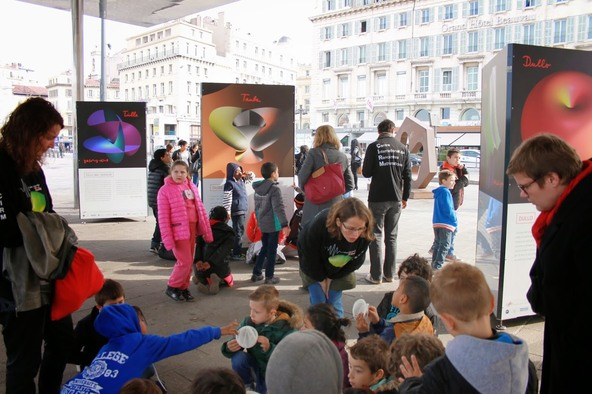
\includegraphics{img/vieux-port-alba.jpg}

Une autre exposition Imaginary à Marseille\\
avec une approche de recherche didactique.
\end{frame}

\hypertarget{questions}{%
\section{Questions?}\label{questions}}

\begin{frame}{Questions?}
\begin{longtable}[]{@{}lll@{}}
\toprule
\endhead
\begin{minipage}[t]{0.32\columnwidth}\raggedright
continuité et ouverture dans la recherche\strut
\end{minipage} & \begin{minipage}[t]{0.29\columnwidth}\raggedright
un vrai souci de l'accessibilité\strut
\end{minipage} & \begin{minipage}[t]{0.30\columnwidth}\raggedright
fibre «maker»\strut
\end{minipage}\tabularnewline
\begin{minipage}[t]{0.32\columnwidth}\raggedright
intérêt en médiation scientifique\strut
\end{minipage} & \begin{minipage}[t]{0.29\columnwidth}\raggedright
enseignement dans le respect\strut
\end{minipage} & \begin{minipage}[t]{0.30\columnwidth}\raggedright
parcours polyvalent\strut
\end{minipage}\tabularnewline
\bottomrule
\end{longtable}

J'ai à cœur de m'intégrer dans la recherche au LAMA et dans
l'enseignement à la FSEG.

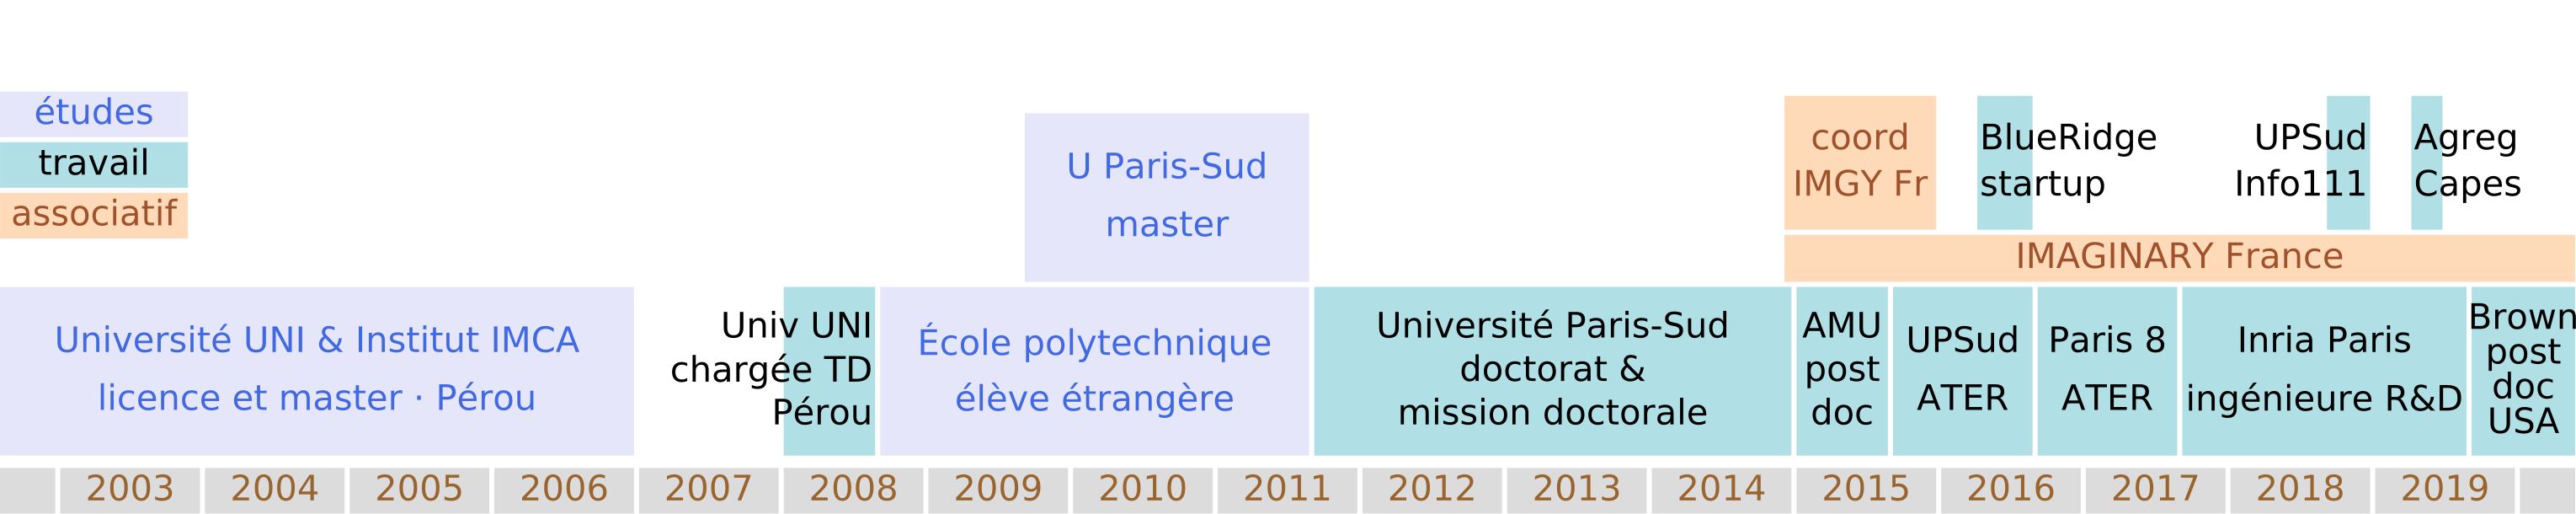
\includegraphics[width=1\textwidth,height=\textheight]{img/alba-timeline.png}
\end{frame}

\end{document}
